%Macros

\documentclass[11pt]{article}
\usepackage{amsmath,amssymb,amsthm}
\usepackage{graphicx}
\usepackage{url}
\usepackage{hyperref}
\usepackage{color}
\usepackage{algorithm,algorithmic}


\newcommand{\INPUT}{\item[{\bf Input:}]}
\newcommand{\OUTPUT}{\item[{\bf Output:}]}
\newcommand{\RR}{{\mathbb R}}
\newcommand{\myvec}[1]{\mathbf{#1}}
\newcommand{\ignore}[1]{}%
\newenvironment{redmatrix}
  {\left(\array{@{}rrrr|c@{}}}
  {\endarray\right)}

\DeclareMathOperator*{\E}{\mathbb{E}}
\let\Pr\relax
\DeclareMathOperator*{\Pr}{\mathbb{P}}
%\DeclareMathOperator*{\myv}{\mathbf{#1}}
\newcommand{\mv}[1]{\mathbf{#1}}
\newcommand{\mynorm}[1]{\|{#1}\|}


\newcommand{\eps}{\varepsilon}
\newcommand{\inprod}[1]{\left\langle #1 \right\rangle}

\newcommand{\handout}[5]{
  \noindent
  \begin{center}
  \framebox{
    \vbox{
      %\hbox to 5.78in { {\bf AM 221: Advanced Optimization } \hfill #2 }
            \hbox to 6.38in { {\bf AM 221: Advanced Optimization } \hfill #2 }
      \vspace{4mm}
      %\hbox to 5.78in { {\Large \hfill #5  \hfill} }
            \hbox to 6.38in { {\Large \hfill #5  \hfill} }
      \vspace{2mm}
            \hbox to 6.38in { {\em #3 \hfill #4} }
      %\hbox to 5.78in { {\em #3 \hfill #4} }
    }
  }
  \end{center}
  \vspace*{4mm}
}

\newcommand{\lecture}[3]{\handout{#1}{#2}{#3}{Lecture #1}}
\newcommand{\homework}[3]{\handout{#1}{#2}{#3}{Problem Set #1}}
\newcommand{\sect}[3]{\handout{#1}{#2}{#3}{Section #1}}

\newtheorem{theorem}{Theorem}
\newtheorem{corollary}[theorem]{Corollary}
\newtheorem{lemma}[theorem]{Lemma}
\newtheorem{observation}[theorem]{Observation}
\newtheorem{proposition}[theorem]{Proposition}
\newtheorem{definition}[theorem]{Definition}
\newtheorem{claim}[theorem]{Claim}
\newtheorem{fact}[theorem]{Fact}
\newtheorem{assumption}[theorem]{Assumption}

\newtheorem*{theorem*}{Theorem}
\newtheorem*{corollary*}{Corollary}
\newtheorem*{conjecture*}{Conjecture}
\newtheorem*{lemma*}{Lemma}
\newtheorem*{thm*}{Theorem}
\newtheorem*{prop*}{Proposition}
\newtheorem*{obs*}{Observation}
\newtheorem*{rem*}{Remark}
\newtheorem*{definition*}{Definition}
\newtheorem{remark}[theorem]{Remark}
\newtheorem*{rec*}{Recommendation}


% 1-inch margins, from fullpage.sty by H.Partl, Version 2, Dec. 15, 1988.
\topmargin 0pt
\advance \topmargin by -\headheight
\advance \topmargin by -\headsep
\textheight 8.9in
\oddsidemargin 0pt
\evensidemargin \oddsidemargin
\marginparwidth 0.5in
\textwidth 6.5in

\parindent 0in
\parskip 1.5ex

%Basics
\newcommand{\new}[1]{{\em #1\/}}		% New term (set in italics).

\newcommand{\boxdef}[1]
{
\fbox{
\begin{minipage}{42em}
\begin{definition*}
{#1}
\end{definition*}
\end{minipage}
}
}

\newcommand{\boxthm}[1]
{
\fbox{
\begin{minipage}{42em}
\begin{theorem*}
{#1}
\end{theorem*}
\end{minipage}
}
}



%Probability
\newcommand{\prob}[2][]{\text{\bf P}\ifthenelse{\not\equal{}{#1}}{_{#1}}{}\!\left(#2\right)}
\newcommand{\expect}[2][]{\text{\bf E}\ifthenelse{\not\equal{}{#1}}{_{#1}}{}\!\left[#2\right]}
\newcommand{\var}[2][]{\text{\bf Var}\ifthenelse{\not\equal{}{#1}}{_{#1}}{}\!\left[#2\right]}

%Sets
\newcommand{\set}[1]{\{#1\}}			% Set (as in \set{1,2,3})
\newcommand{\given}{\, : \,}
\newcommand{\setof}[2]{\{{#1} \given {#2}\}}	% Set (as in \setof{x}{x > 0})
\newcommand{\compl}[1]{\overline{#1}}		% Complement of ...            
\newcommand{\zeros}{{\mathbf 0}}
\newcommand{\ones}{{\mathbf 1}}
\newcommand{\union}{{\bigcup}}
\newcommand{\inters}{{\bigcap}}

%Other Math
\newcommand{\floor}[1]{{\lfloor {#1} \rfloor}}
\newcommand{\bigfloor}[1]{{\left\lfloor {#1} \right\rfloor}}
\DeclareMathOperator{\argmax}{argmax}
\DeclareMathOperator{\argmin}{argmin}

\newcommand{\PRIMAL}{{\textsc{Primal }}}
\newcommand{\DUAL}{{\textsc{Dual }}}



%Numbers
\newcommand{\C}{\mathbb{C}}	                % Complex numbers.
\newcommand{\N}{\mathbb{N}}                     % Positive integers.
\newcommand{\Q}{\mathbb{Q}}                     % Rationals.
\newcommand{\R}{\mathbb{R}}                     % Reals.
\newcommand{\Z}{\mathbb{Z}}                     % Integers.
\newcommand{\M}{\mathcal{M}}                     % Matroids.
\newcommand{\I}{\mathcal{I}}                     % Independent Sets.

%Headings
\newcommand{\parta}{\textbf{(a)}}
\newcommand{\partb}{\textbf{(b)}}
\newcommand{\partc}{\textbf{(c)}}
\newcommand{\partd}{\textbf{(d)}}
\newcommand{\parte}{\textbf{(e)}}

\newcommand{\bt}{\boldsymbol{\theta}}
\newcommand{\bx}{\mathbf{x}}
\newcommand{\bd}{\mathbf{d}}
\newcommand{\by}{\mathbf{y}}
\newcommand{\bv}{\mathbf{v}}
\newcommand{\bz}{\mathbf{z}}
\newcommand{\bh}{\mathbf{h}}
\newcommand{\ba}{\mathbf{a}}
\newcommand{\cl}[1]{\text{\textbf{#1}}}
\newcommand{\eqdef}{\mathbin{\stackrel{\rm def}{=}}}


\begin{document}
\homework{2 --- {\color{red} Due Wed, Feb 7th at 23:59}}{Spring
  2018}{Kojin Oshiba}

%\renewcommand{\abstractname}{}
\paragraph{Instructions:}
All your solutions should be prepared in \LaTeX \ and the
PDF and .tex should be submitted to canvas. For each question, the best and
correct answers will be selected as sample solutions for the entire class to
enjoy.  If you prefer that we do not use your solutions, please indicate this
clearly on the first page of your assignment. 

The programming parts can be written in the programming language of your choice
and the code should be submitted alongside your solutions.
\newline

\paragraph{1. Convex Sets.} Prove or give a counterexample:
\begin{itemize}
\item [a.] The intersection of convex sets is a convex set.
\item [b.] A half-space is a convex set.
\item [c.] Every polyhedron is a convex set (remember that a polyhedron is the
    feasible set of a linear program, \emph{i.e.} it is defined by a finite set
    of linear inequalities)
\end{itemize}

\color{blue}
\begin{itemize}
\item [a.] If the intersection is an empty set or has a single element, the intersection is convex by definition. If not, take any two points in the intersection. Since the two points must be contained in the same convex set (because we are taking the intersection), the intersection must be convex.
\item [b.] WLOG, let the half space be $H=\{\bx \in \mathbb{R}^n: \ba^T \bx \geq \alpha\}$. Let $\bx_1,\bx_2 \in H$. Then, $\forall \lambda \in [0,1]$
\begin{align*}
\ba^T(\lambda \bx_1 + (1-\lambda) \bx_2) &= \lambda \ba^T \bx_1 + (1 - \lambda) \ba^T \bx_2 &\\
& \geq \lambda \alpha + (1 - \lambda) \alpha = \alpha, 
\end{align*}
Hence, $\lambda \bx_1 + (1-\lambda) \bx_2 \in H, \forall \lambda \in [0,1]$. Therefore, it is a convex set.
\item [c.] Polyhedron can be defined as $P=\{\bx \in \mathbb{R}^n: A\bx \leq \textbf{b} \}$ for some $A\in \mathbb{R}^{m\times n}$ and some $\textbf{b} \in \mathbb{R}^m$.
Note that $P=\{\bx \in \mathbb{R}^n: \ba_1^T \bx \leq \textbf{b}, \ba_2^T \bx \leq \textbf{b}, ..., \ba_n^T \bx \leq \textbf{b} \}$.
This means that polyhedron is an intersection of half spaces. Since in $\ba,\textbf{b}$, we showed that the intersection of convex sets are convex and that half spaces are convex, we have that polyhedron is convex.
\end{itemize}
\color{black}

\paragraph{2. Convex Hulls.}

Let us define the \emph{convex hull} of a set $X$ as the smallest (for the
partial order defined by inclusion) convex set containing $X$ and denote it by
$C(X)$. In other words, there is no other convex set $C'$ such that $X\subseteq
C'\subset C(X)$.

\begin{itemize}
    \item[a.]  Show that $C(X)$ is the intersection of all convex sets
        containing $X$ that is:
        \begin{displaymath}
            C(X) = \bigcap \left \{ C \,|\, X\subseteq C \text{ and } C \text{
            is convex}\right\}
        \end{displaymath}
    \item[b.] What is the convex hull of a convex set?
    \item[c.]
        Show that when $X = \{\bx_1,\ldots,\ldots \bx_n\}$ is finite, then
        $C(X)$ can also be written as: \begin{displaymath} C(X)
            = \left\{\sum_{i=1}^n \lambda_i \bx_i\;|\;\lambda_i\geq 0,\;1\leq
            i\leq n\text{ and } \sum_{i=1}^n \lambda_i=1\right\}
        \end{displaymath}
    \item [d.] What is the convex hull of two points? three points?
\end{itemize}

\color{blue}
\begin{itemize}
\item [a.] Let $Z = \bigcap \{C| \text{$X \subseteq C$ and $C$ is convex}\}$. $Z$ is convex because it is an intersection of convex sets. Suppose $Z \neq C(X)$. Then, there exists a convex set $C'$ such that $X \subseteq C' \subset Z$. However, from how $Z$ is defined, it must be the case that $Z \subseteq C'$. Hence, contradiction. Therefore, $Z=C(X)$.
\item [b.] Convex hull of a convex set is itself.
\item [c.] Let $Comb(X) = \{\sum_{i=1}^n \lambda_i \bx_i | \lambda_i \geq 0, 1 \leq i \leq n, \sum_{i=1}^n \lambda_i = 1 \}$. We would like to show that $C(X)=Comb(X)$. First we show that $Comb(X) \subseteq C(X)$. To show this, it suffices to show that if a set $C$ is convex, then any convex combination of points in $C$ is in $C$. We prove this by induction.
$n=1$ is trivial. $n=2$ follows from the definition of convex sets.
Suppose, for $n=k$, we have $\bx = \sum_{i=1}^k \lambda_i \bx_i \in C$, where $\bx_1, ..., \bx_k \in C, \sum_{i=1}^k \lambda_i = 1, \lambda_i \geq 0 \forall i$ 
Then, for $n=k+1$, 
\begin{align*}
\bx &= \sum_{i=1}^{k+1} \lambda_i \bx_i &\\
&= \sum_{i=1}^k \lambda_i \bx_i + \lambda_{k+1} \bx_{k+1} &\\
&= (1 - \lambda_{k+1}) \sum_{i=1}^k \frac{\lambda_i}{1-\lambda_{k+1}}\bx_i + \lambda_{k+1} \bx_{k+1} 
\end{align*}
Because $\sum_{i=1}^k \frac{\lambda_i}{1-\lambda_{k+1}} = 1, \frac{\lambda_i}{1-\lambda_{k+1}} \geq 0 \ \forall i, \sum_{i=1}^k \frac{\lambda_i}{1-\lambda_{k+1}} \bx_i \in C$
Hence, $\bx$ is also in $C$. Therefore, we have $Comb(X) \subseteq C(X)$.

By setting $\lambda_i=1$ and the rest to $0$ for $\bx_i \in \bx$, $X \subseteq Comb(X)$. So, all we need to show now is that $Comb(X)$ is convex.
Let $y,z \in Comb(X)$ and $y=\sum_i \ba_i \bx_i, z=\sum_i \textbf{b}_i \bx_i$. Then,

$cy+(1-c)z = c\sum_i \ba_i \bx_i + (1-c) \sum_i \textbf{b}_i \bx_i = \sum_i \bd_i \bx_i$ where $\bd_i = c\ba_i + (1-c) \textbf{b}_i$.
Hence, $c y + (1-c) z \in Comb(X)$.
\item [d.] Convex hull of two points is the straight line connecting the two points. Convex hull of three points is inside of the triangle (edge inclusive) where the three points correspond to the vertices.
\end{itemize}
\color{black}

\paragraph{3. Strict Convexity of the $\ell_2$ norm.}

Let $y$ be an arbitrary point in $\mathbb{R}^n$ and let us define the function
``distance to y'' by:
\begin{displaymath}
    d_{\by}(\bx) = \|\bx-\by\|_2^2,
    \quad \bx\in\mathbb{R}^n
\end{displaymath}
Show that the function $d_{\by}$ is strictly convex. Remember that a function $f$
defined over $\mathbb{R}^n$ is strictly convex if and only if for any pair of
points $\bx, \by\in\mathbb{R}^n$ with $\bx\neq \by$ and any $\lambda\in(0,1)$:
\begin{displaymath}
    f\big(\lambda \bx + (1-\lambda)\by\big) < \lambda f(\bx) + (1-\lambda) f(\by)
\end{displaymath}
\color{blue}
\begin{align*}
d_{\by}(\lambda\bx_1+(1-\lambda)\bx_2) &= \|\lambda \bx_1+(1-\lambda)\bx_2-\by\|_2^2 &\\
&= \|\lambda (\bx_1-\by)+(1-\lambda)(\bx_2-\by)\|_2^2 &\\
&\leq (\|\lambda (\bx_1-\by)\|_2+\| (1-\lambda)(\bx_2-\by) \|_2)^2 \ (\because \text{triangle inequality}) &\\
&= (\lambda \| \bx_1-\by\|_2+(1-\lambda) \| \bx_2-\by \|_2)^2  &\\
&< \lambda \| \bx_1-\by\|_2^2 + (1-\lambda) \| \bx_2-\by \|_2^2  \ (\because \text{strict convexity of the quadratic})
\end{align*}
\color{black}
\paragraph{4. Infeasibility and Unboundedness.} 

Discuss the feasibility and boundedness of the following linear programs:
\begin{alignat*}{4}
    &\text{maximize }   & 2x_2 + x_3&  &\qquad\qquad&\text{minimize}&x+y+z+w&\\
    &\text{subject to } & x_1 - x_2 &\leq 5&\qquad\qquad&\text{subject to}&x+3y+2z+4w&\leq 5\\
    &                   & -2x_1 + x_2 &\leq 3&\qquad\qquad&&3x+y+2z+w&\leq 4\\
    &                   & x_1 - 2x_3&\leq 5&\qquad\qquad&&5x+3y+3z+3w&=9\\
    &                   &x_1, x_2, x_3&\geq 0&\qquad\qquad&&x, y, z, w&\geq 0\\
\end{alignat*}
\color{blue}
\textbf{First LP}

Let 
$A = 
\begin{pmatrix}
1 & -1 & 0 \\
-2 & 1 & 0 \\
1 & 0 & -2 
\end{pmatrix}$,
$\bx = 
\begin{pmatrix}
\bx_1 \\
\bx_2 \\
\bx_3
\end{pmatrix}$,
$\textbf{b} = 
\begin{pmatrix}
5 \\
3 \\
5
\end{pmatrix}$.

$A\bx = \textbf{b}$ has a single solution $\bx = \begin{pmatrix}
-8 \\
-13 \\
-6.5
\end{pmatrix}$.
However, this doesn't satisfy $\bx \geq 0$. Hence from Farka's lemma, this LP is infeasible. We can't really discuss boundedness here since LP is infeasible.

\textbf{Second LP}

Let 
$A = 
\begin{pmatrix}
-1 & -3 & -2 & -4 \\
-3 & -1 & -2 & -1 \\
-5 & -3 & -3 & -3 \\
5 & 3 & 3 & 3 \\ 
\end{pmatrix}$,
$\textbf{b} = 
\begin{pmatrix}
-5 \\
-4 \\
-9 \\
9
\end{pmatrix}$,
$\textbf{c} = 
\begin{pmatrix}
1 \\
1 \\
1 \\
1
\end{pmatrix}$.

Then the primal LP can be written as:

$min \ \textbf{c}^T \bx$, subject to $A\bx \geq \textbf{b}$.

Then, the dual LP can be written as:

$max \ \textbf{b}^T \by$ subject to $A^T \by = \textbf{c}, \by \geq 0$

Since row-echelon form of $A$ can be written as
$
\begin{redmatrix}
1&0&0&-0.375&0\\
0&1&0&1.125&0.25\\
0&0&1&0.5&-1\\
0&0&0&0&2
\end{redmatrix}
$,

$A^T \by = \textbf{c}$ doesn't have a solution. Hence, this dual LP is infeasible.

From strong duality, if dual LP is infeasible, primal is either infeasible or unbounded. But since we have that the primal is feasible, it must be the case that the primal is unbounded.
\color{black}

\paragraph{5. Linear Classifiers and the Perceptron Algorithm}

In this problem, we will work on the Iris dataset available at
\url{https://archive.ics.uci.edu/ml/machine-learning-databases/iris/iris.data}.
The dataset is a single comma-separated value (CSV) file. The first 4 fields of
each line contain the measurements of a sample of Iris flower, the
last field is the name of this sample's species of Iris. More information about
the dataset can be found at
\url{https://archive.ics.uci.edu/ml/machine-learning-databases/iris/iris.names}.

The goal of this problem is to construct a classifier to distinguish the
\emph{Iris setosa} from the other species of Iris. That is, we want to construct
a function $f$ which takes as input the vector $\bx\in\mathbb{R}^4$ of
measurements of a sample and return $f(\bx)\in\{0,1\}$ such that:
\begin{displaymath}
    f(\bx) = \begin{cases}
        1& \text{if the sample is an Iris setosa}\\
        0& \text{otherwise}
    \end{cases}
\end{displaymath}

\begin{itemize}
    \item[a.] Download the dataset, choose a pair of coordinates (that is, any
        two of the first four fields) and draw a scatter plot of the dataset
        for this pair of coordinates. The color of the points should be
        determined by the Iris species.
    \item[b.] Are the samples of Iris setosa linearly separable (that is, does
        there exist a separating hyperplane) from the samples from the other
        species? Is a linearly separable dataset always separable after having
        been projected on an arbitrary pair of coordinates? (prove of describe
        a counter-example)?
    \item[c.] Explain why finding a separating hyperplane as described in the
        previous part is sufficient to construct a classifier $f$ as
        described in the introduction of this problem. A classifier constructed
        in such a way is called a \emph{linear classifier}.
    \item[d.] Implement the perceptron algorithm in the programming language of
        your choice. Run your algorithm on the Iris dataset to find
        a hyperplane separating the Iris setosa samples from the other samples.
        Report the weights defining the hyperplane as well as the code you
        wrote.
\end{itemize}

\color{blue}
\begin{itemize}
\item[a.] I chose the first two coordinates.

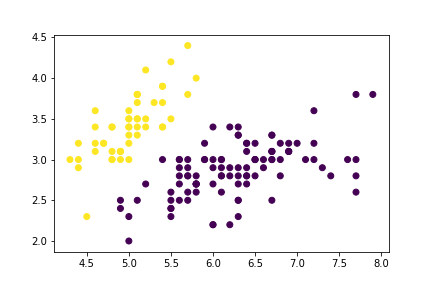
\includegraphics[scale=0.8]{iris}
\item[b.] To answer the first question, yes, it is linearly separable because it is linearly separable in a subset of all features. To answer the second question, not necessarily. Even if the data is linearly separable given all features, it does not mean that it is liearly separable in the projected space. Consider a separating (hyper)plane in 3D space that is parallel to the x and y axes. Then the data is clearly separable in 3D, but when project onto the x-y 2D plane, the data is no longer seperable if, say one point from two clusters have the same x,y coordinates (but different z coordinate).
\item[c.] Because $f(\bx)$ can be defined as an indicator variable that returns 1 if a data point is above the hyperplane and 0 otherwise. If the hyperplane completely separates the two labels, then that means that $f$ classifies the datapoints entirely.
\item[d.] The weights are [-0.03152507, -0.19633574,  0.29397583,  0.12135334,  0.04675983]. The code is in `hw2.py`.
\end{itemize}
\color{black}


\end{document}
